\documentclass[10pt,a4paper,final]{article}
\usepackage[utf8]{inputenc}
\usepackage[fixlanguage]{babelbib}
\usepackage[english]{babel}
\usepackage{amsmath}
\usepackage{amsfonts}
\usepackage{amssymb}
\usepackage[left=2cm,right=2cm,top=2cm,bottom=2cm]{geometry}
\usepackage[round,sort,nonamebreak]{natbib} % citação 

\usepackage[usenames,svgnames,dvipsnames]{xcolor}
\usepackage[pdftex]{graphicx}           % usamos arquivos pdf/png como figuras
\usepackage{float}%To make tables and figures stay where we want
\graphicspath{{./figures/}}



\title{Numerical Inverse Laplace Transform Integration on Ellipses}
\author{Pedro S. Peixoto}

\begin{document}
\maketitle

\section{Numerical Inverse Laplace Transform Integration on a Circle}


Inverse Laplace Transform (via Bromwich integral),
\begin{equation}
{ \mathfrak{ L } }^{ -1 }\left\{ \widehat { f }  \right\} =\frac { 1 }{ 2\pi i } \int _{ \gamma -i\infty  }^{ \gamma +i\infty  }{ { e }^{ st }\widehat { f } \left( s \right) ds } .
\end{equation}
From the Residual Theorem we can replace it with 
\begin{equation}
{ \mathfrak{ L } }^{ -1 }\left\{ \widehat { f }  \right\}=\frac{1}{2\pi i}\int _{ { C }^{  } }{ { e }^{ st }\widehat { f } \left( s \right) ds },
\end{equation}
as long as all the poles of $\widehat{f}$ lay inside a closed contour ($C$). Following \citet{cclancy11} and \citet{clancy:PhD} one can choose a circle centered at the origin and of radius $\gamma$.
\begin{figure}[!h]
  \centering
  \hspace{1cm}
  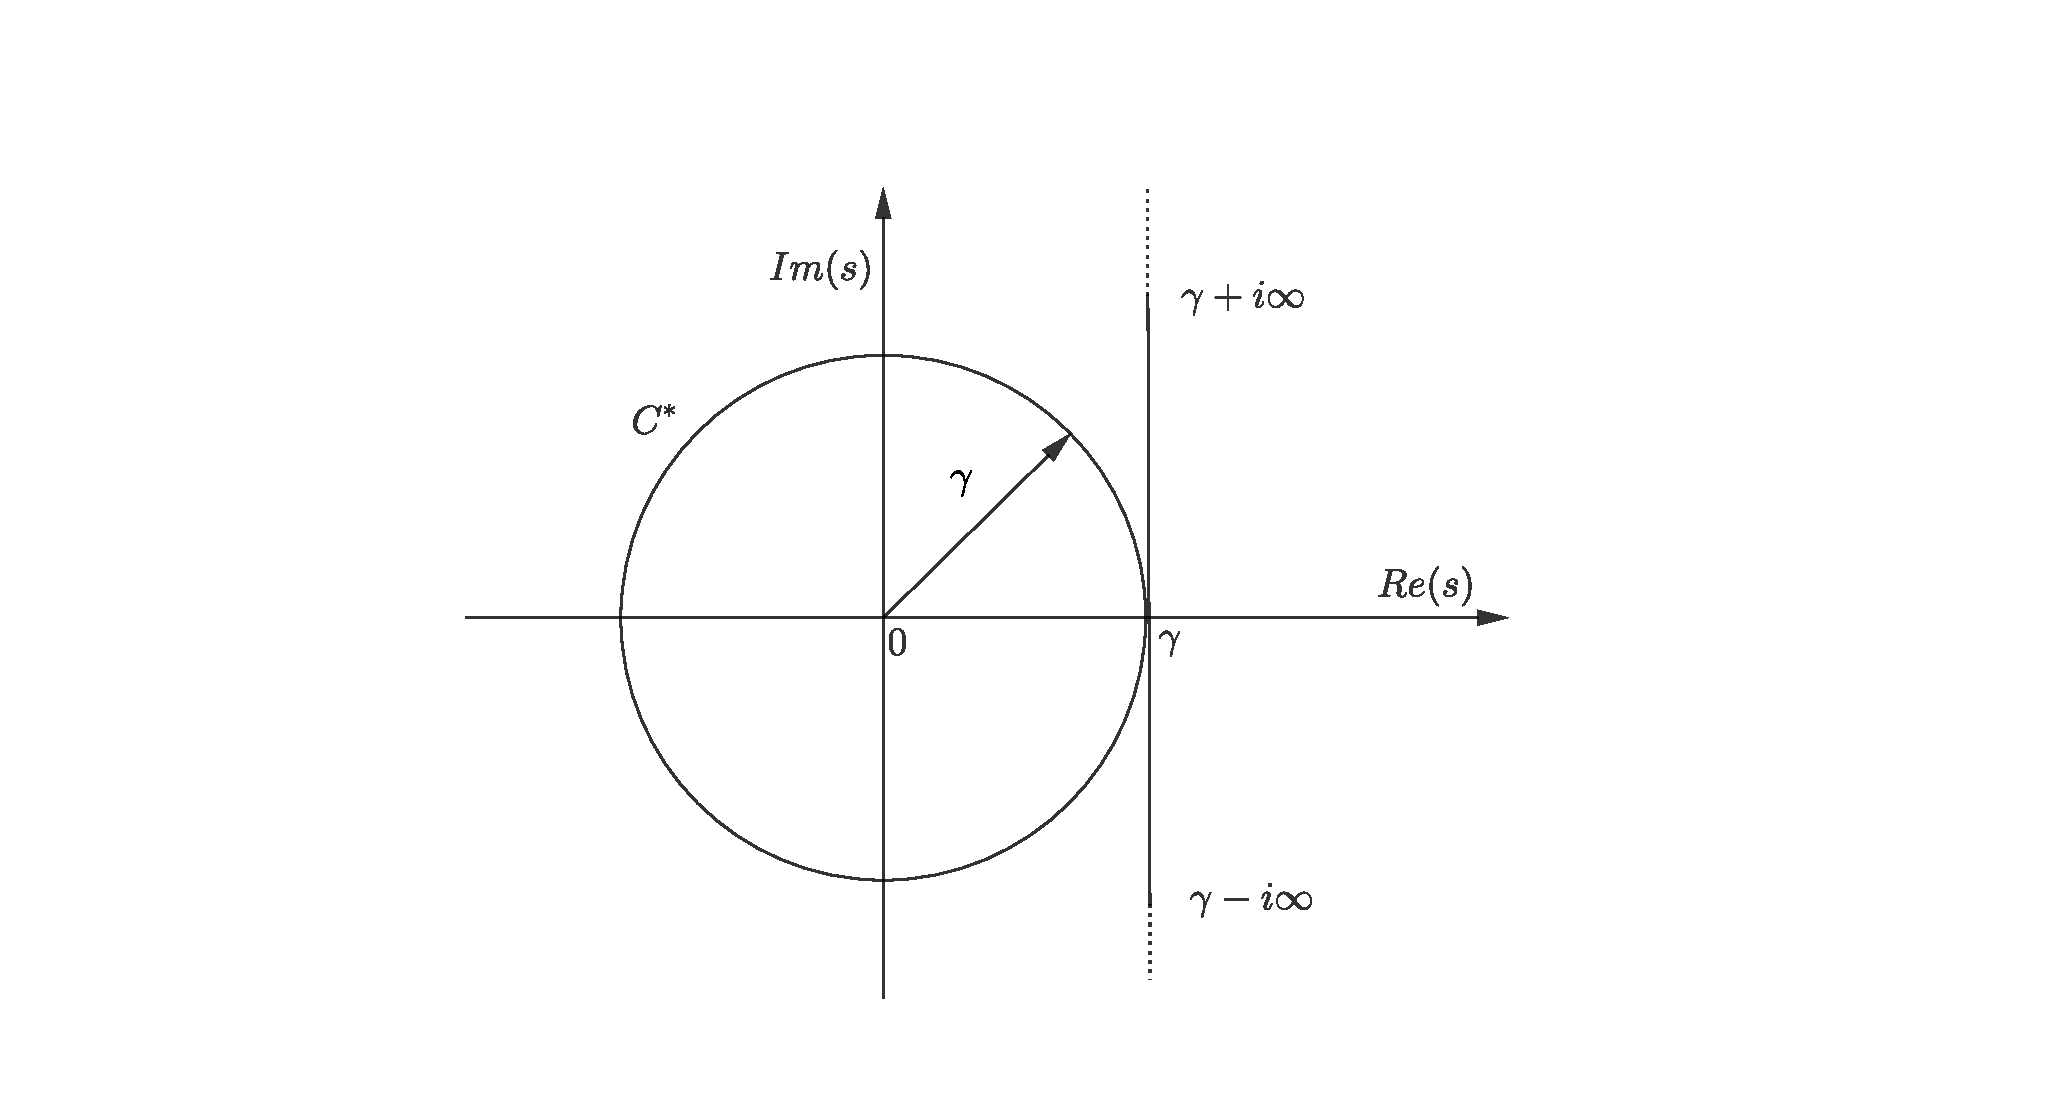
\includegraphics[width=.5\textwidth]{Cstar} 
  \caption[Closed contour $C $]{Closed contour $C$}
  \label{fig:Cstar} 
\end{figure}

The integral over the contour $C $ can be solved using the parametrized circle $s(\theta)=\gamma e^{i\theta}$, $\theta \in [0,2\pi]$.
\begin{equation}
{ \mathfrak{ L } }^{ -1 }\left\{ \widehat { f }  \right\}=\frac{1}{2\pi i}\int _{ { C }^{  } }{ { e }^{ st }\widehat { f } \left( s \right) ds }=\frac{1}{2\pi i}\int _{0}^{2\pi}{ { e }^{ s(\theta)t }\widehat { f } \left( s(\theta) \right)s'(\theta) ds },
\end{equation}
where $s'(\theta)=is(\theta)$. This integral can be approximated via numerical quadrature, using Trapezoidal Rule, on the $N$  points $\theta_n=2\pi n/N$, that results in 
\begin{equation}
{ \mathfrak{ L } }^{ * }_C\left\{ \widehat { f }  \right\}=\frac { 1 }{ Ni} \sum _{ n=1 }^{ N }{ { e }^{ { s }_{ n }t }\widehat { f } \left( { s }_{ n } \right) { s }'_{ n } }
\end{equation}
where,
\begin{equation}
s_{n}=\gamma e^{{i\theta_n}}, \quad s'_{n}=\gamma i e^{{i\theta_n}}=is_n.
\end{equation}

\section{Numerical Inverse Laplace Transform Integration on an Ellipse}

Now we wish to use an ellipse $E $ instead of a circle $C $ as closed contour. This ellipse will be chosen to satisfy the following properties:\\
(i) On the imaginary axis, it will be bounded by the interval $[-\gamma, \gamma]$, for $\gamma >0$.\\
(ii) On the real axis it will be bounded by the interval $[-\delta, \delta]$, where $\delta < 1$.

The first requirement ensures we can solve hyperbolic with purely imaginary eigenvalues up to the frequency defined by $\gamma$. The second requirement ensures that having larger timestep sizes in the numerical time integration will not lead to evaluations of complex functions with large real parts, avoiding floating point instabilities.

\subsection{Parameterized ellipse}

To attend the above requirements, the ellipse may be defined via specialized Joukowsky transforms. Let $\theta \in [0,2\pi]$ and $z=re^{i\theta}$ define a circle of radius $r$ on the complex plane. An ellipse, following the above requirements, maybe built as function of $\theta$ with the Joukowsky transform
\begin{equation}
w(\theta)=\frac{\gamma i}{d}\left(re^{i\theta}+\frac{e^{-i\theta}}{r}\right),
\end{equation}
where $d>0$ is yet to be determined. The $i\gamma/d$ term in the Joukowsky is responsible for a few things: $i$ shifts rotates the ellipse, so that its larger axis is placed in the imaginary axis; $\gamma/d$ is a normalization to allow that request (i) is satisfied. 

The first condition (i) imposes that
\begin{equation}
|\text{Im}(w(\theta))|= \frac{\gamma }{d}\left(r+\frac{1}{r}\right)|\cos(\theta)| \leq \gamma, \quad \forall \theta \in [0, 2\pi].
\end{equation}
In the Joukowsky transform, when $r=1$, the ellipse degenerates to a line segment, in this case the interval $[-2\gamma i/d, 2\gamma i/d]$. Choosing 
\begin{equation}
d=\left(r+\frac{1}{r}\right),
\end{equation}
is enough to fulfill condition (i).

To fulfill condition (ii), $r$ needs to be chosen such that 
\begin{equation}
|\text{Re}(w(\theta))|=\frac{\gamma}{d}|(r^{-1}-r)\sin(\theta)|\leq\delta <1 , \quad \forall \theta \in [0, 2\pi].
\end{equation}
A condition for this to happen, already using that $d=r^{-1}+r$, is that
\begin{equation}
\frac{|r^{-1}-r|}{r^{-1}+r}<\delta /\gamma
\end{equation}
which, for $r>0$, is illustrated in the figure below.

\begin{figure}[h!]
\centering
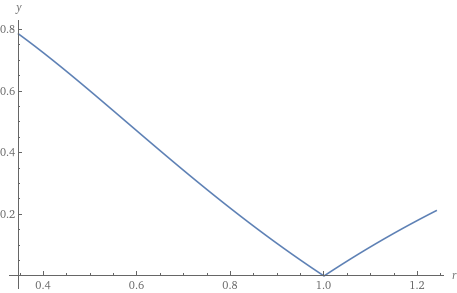
\includegraphics[scale=0.7]{rlimits1}
\caption{$\frac{|r^{-1}-r|}{r^{-1}+r}$}
\end{figure}

Therefore, condition (ii) is satisfied if 
\begin{equation}
\sqrt{\frac{1-\delta/\gamma}{1+\delta/\gamma}} <r<\sqrt{\frac{1+\delta/\gamma}{1-\delta/\gamma}}. 
\end{equation}

To avoid degenerate ellipses, we need $r\neq 1$. The symmetry around $r=1$ of the Joukowsky transform allows us to freely chose either $r>1$ or $r<1$. Here, we choose
\begin{equation}
r=\sqrt{\frac{1-\delta/\gamma}{1+\delta/\gamma}},
\end{equation}
which is adequate to ensure the imposed conditions.


With $\gamma=2$, $\delta=1$ (in practice $\delta$ should be strictly smaller than $1$, but this is just an illustration) the ellipse generated would look like the figure bellow. 
\begin{figure}[h!]
\centering
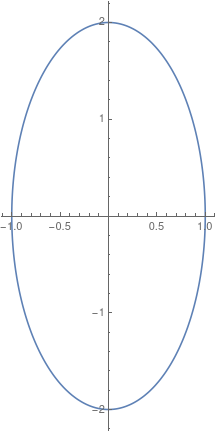
\includegraphics[scale=0.6]{ellipse.png}
\label{fig:ellip2_1}
\end{figure}




\subsection{Inverse Laplace Transform}
Lets now go back to the Inverse Laplace Transform, but now with the contour defined via the ellipse contour. 

Using the properties of contour integration, the Inverse Laplace transform on the ellipse maybe written as
\begin{equation}\label{MILT_ellipse}
{ \mathfrak{ L } }^{ -1 }\left\{ \widehat { f }  \right\}=\frac{1}{2\pi i}\int _{ { E }^{  } }{ { e }^{ st }\widehat { f } \left( s \right) ds }=\frac{-1}{2\pi i}\int_{0}^{2\pi} e^{s(\theta)t}\widehat { f } \left( s(\theta) \right) s'(\theta)\,d\theta,
\end{equation}
where 
\begin{equation}
s(\theta)=\frac{\gamma i}{d}\left(re^{i\theta}+\frac{e^{-i\theta}}{r}\right),
\end{equation}
and
\begin{equation}
s'(\theta)=-\frac{\gamma}{d}\left(re^{i\theta}-\frac{e^{-i\theta}}{r}\right),
\end{equation}
and the minus sign in the integration ensures the contour is swept in a counter-clockwise way.

Uniformly partitioning the $[0,2\pi]$ interval on $N$ points with $\theta_n=2\pi n/N$, we may define the complex quadrature points as
\begin{equation}
s_n=\frac{\gamma i}{d}\left(re^{i\theta_n}+\frac{e^{-i\theta_n}}{r}\right), \quad n=1,2,..,N,
\end{equation}
and respectively the metric terms as
\begin{equation}
s'_n=-\frac{\gamma}{d}\left(re^{i\theta_n}-\frac{e^{-i\theta_n}}{r}\right),  \quad n=1,2,..,N.
\end{equation}

\begin{figure}[h!]
\centering
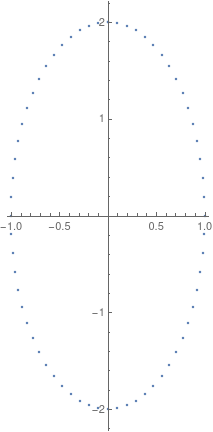
\includegraphics[scale=0.4]{ellipse-quadpoints64}
\caption{64 quadrature points on an ellipse with $\gamma=2$ and $\delta=1$.}
\end{figure}

The quadrature points are not uniformly (equidistantly) distributed on the ellipse contour. However, the $\theta_n$ points are equidistantly distributed on the $[0,\pi]$ interval, ensuring exponential convergence of the Trapezoidal Rule, for instance, of the following estimate for the inverse Laplace transform

\begin{equation}\label{milt_ellipse}
{ \mathfrak{ L } }^{ * }_E\left\{ \widehat { f }  \right\}=-\frac { 1 }{  N i} \sum _{ n=1 }^{ N }{ { e }^{ { s }_{ n }t }\widehat { f } \left( { s }_{ n } \right) { s }'_{ n } }
\end{equation}

\section{Constant reconstruction}

Let $\widehat{f}(s)=1/s$, such that $f(t)=1$. Then the following equalities should hold (approximately):

\begin{equation}
{ \mathfrak{ L } }^{ * }_C\left\{ 1/s \right\}=\frac { 1 }{ Ni} \sum _{ n=1 }^{ N }{ { e }^{ { s }_{ n }t }{ s }'_{ n } /s_n} \approx 1,
\end{equation}

\begin{equation}\label{milt_ellipse}
{ \mathfrak{ L } }^{ * }_E\left\{ 1/s  \right\}=-\frac { 1 }{  Ni} \sum _{ n=1 }^{ N }{ { e }^{ { s }_{ n }t }{ s }'_{ n }/s_n }\approx 1.
\end{equation}
where $s_n$ and $s'_n$ are defined differently on the circle and ellipse, as defined in the previous sections.

This reconstruction should be independent on $t$ (which will be our $dt$ in the ODE integration scheme).

We have set the a circle with radius $10$ and an ellipse with $\gamma=10$ and $\delta=0.5$, as the figure bellow.
\begin{figure}[h!]
\centering
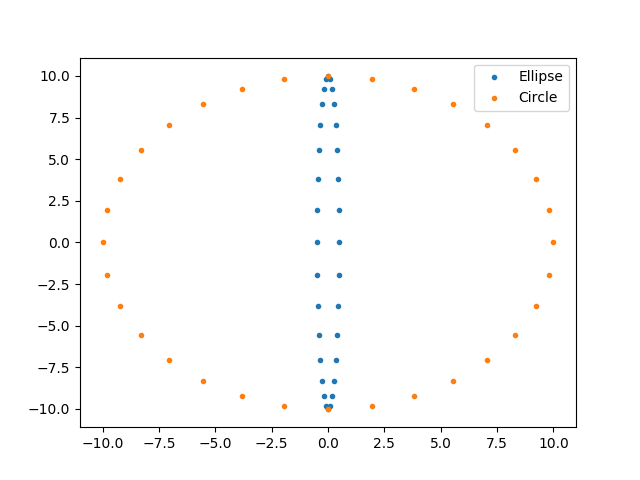
\includegraphics[scale=0.5]{ellip_circ}
\label{fig:quad_elip_circ}
\caption{Quadrature points for circle ($\gamma=10$) and ellipse ($\gamma=10$, $\delta=0.5$) with $N=32$}
\end{figure}


The results bellow indicate how the circle provides an accurate reconstruction for small $dt$, but how it breaks down due to floating point errors when large $dt$ are used. The ellipse has larger errors, but allows larger $dt$.

\begin{figure}
\centering

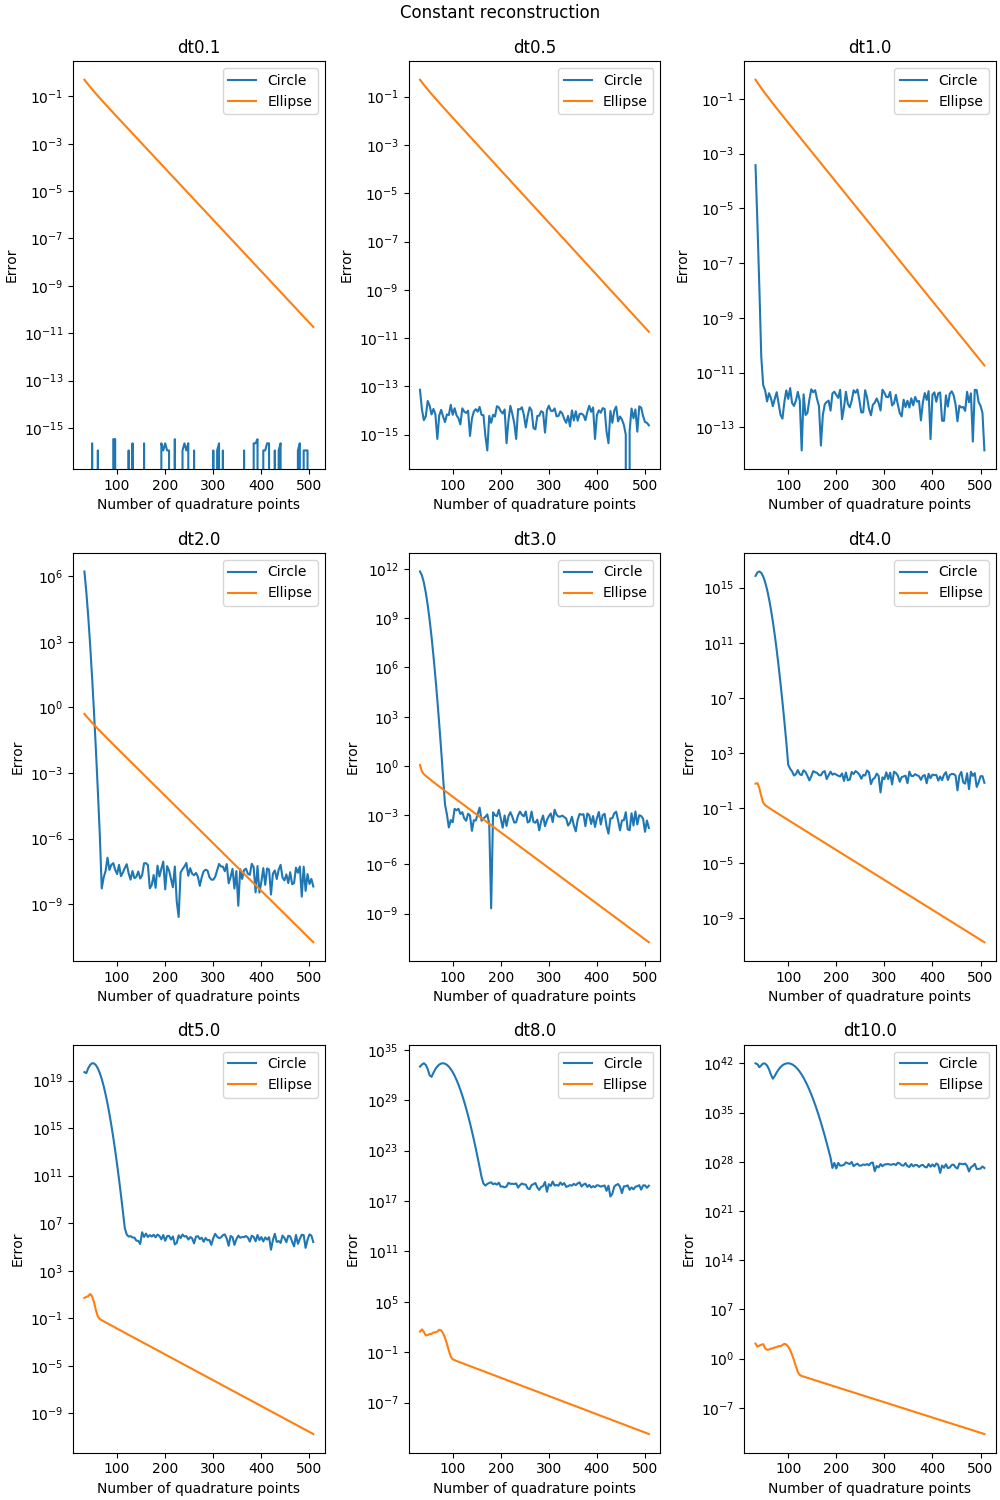
\includegraphics[scale=0.5]{const_recon}
\label{fig:const}
\caption{Absolute error in the numerical inversion of the function $\widehat{f}=1/s$, which should result in $f(t)=1$ for any $t$ ($dt$). }
\end{figure}


\clearpage 
\section{Exponential truncation}


\citet{cclancy11} and \citet{clancy:PhD} use a truncated Taylor series in the calculation of the exponential term,
\begin{equation}
{e }^{ { s }_{ n }t }=\sum_{j=0}^{N}\frac{(s_nt)^j}{j!},
\end{equation}
with $N$ matching the number of quadrature points. For the contour integration  on a circle, \citet{clancy:PhD} showed that the truncated series, with $N$ even, leads to exact reconstructions of polynomials, that is, 
\begin{equation}
\mathfrak{ L }^{ * }_C\left(\frac{1}{s^{k+1}}\right)=\frac{t^k}{k!}, \quad 0\leq k \leq N.
\end{equation}

We explored numerically the effects of having the truncated exponential and the results are shown in  Figures \ref{fig:const_truncN} and \ref{fig:const_trunc16}, that show the errors when the exponential series is truncated with $N$ and $16$ terms respectively. The exponential series is highly sensitive to numerical floating point precision, therefore, for large $dt$, it creates numerical instabilities in both the Circle and Ellipse contours. Reducing the number of terms in the exponential series expansion (to 16) alleviates the problem of numerical stability on the circle, but deteriorates the results for the ellipse.

\begin{figure}[h!]
\centering
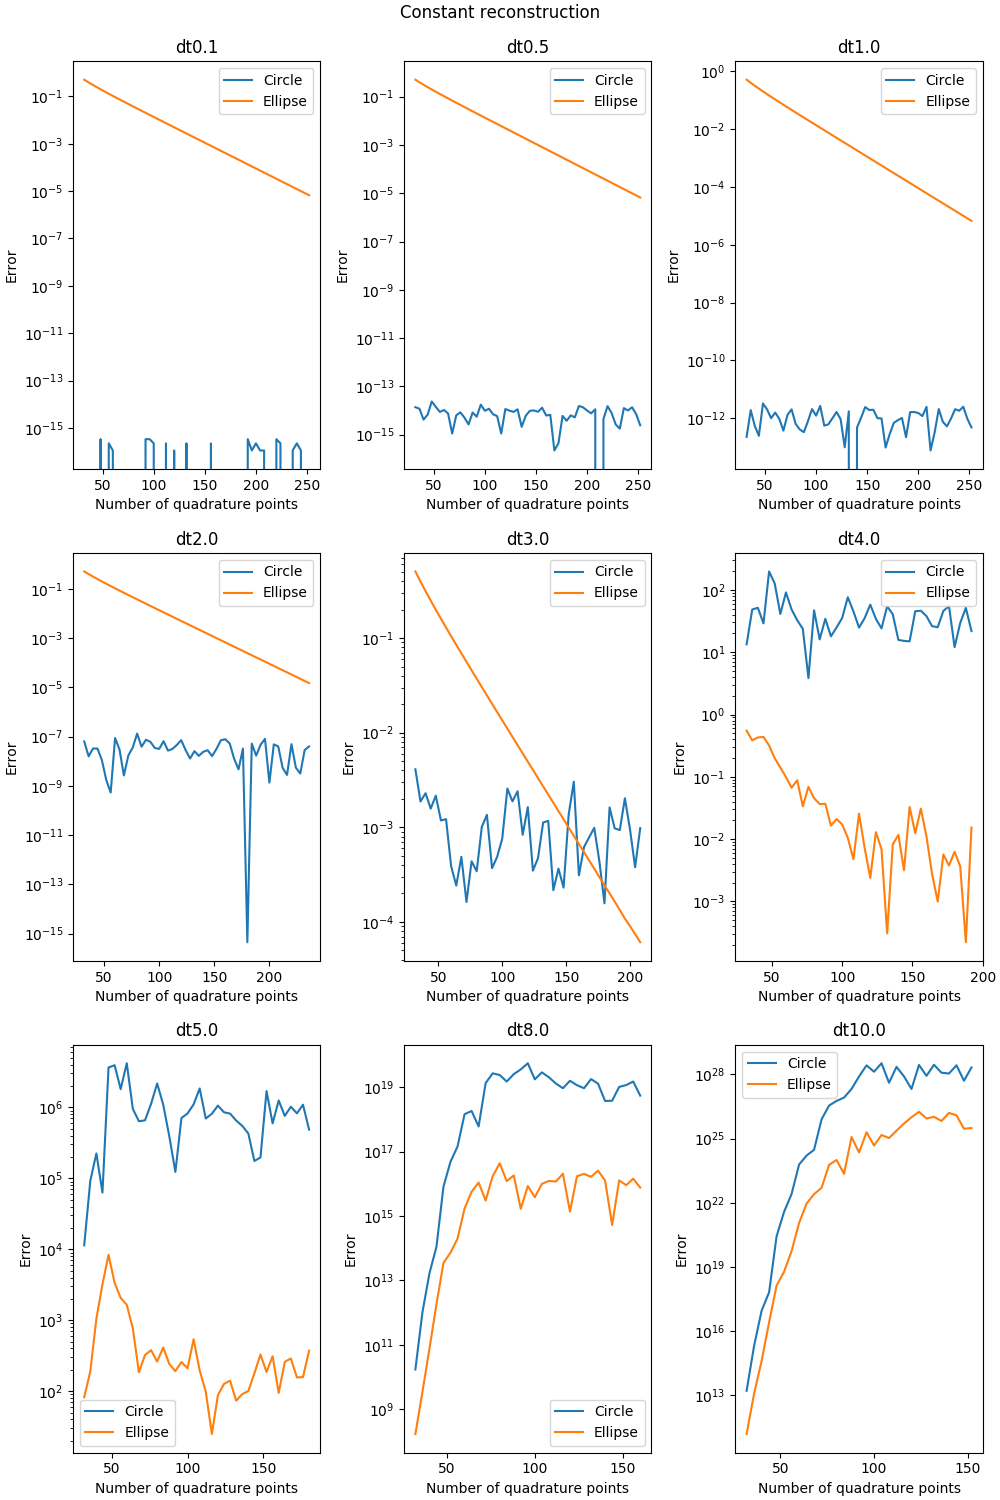
\includegraphics[scale=0.5]{const_recon_truncN}
\label{fig:const_truncN}
\caption{Absolute error in the numerical inversion of the function $\widehat{f}=1/s$ using truncated exponential with $N$ terms, which should result in $f(t)=1$ for any $t$ ($dt$). }
\end{figure}


\begin{figure}[h!]
\centering
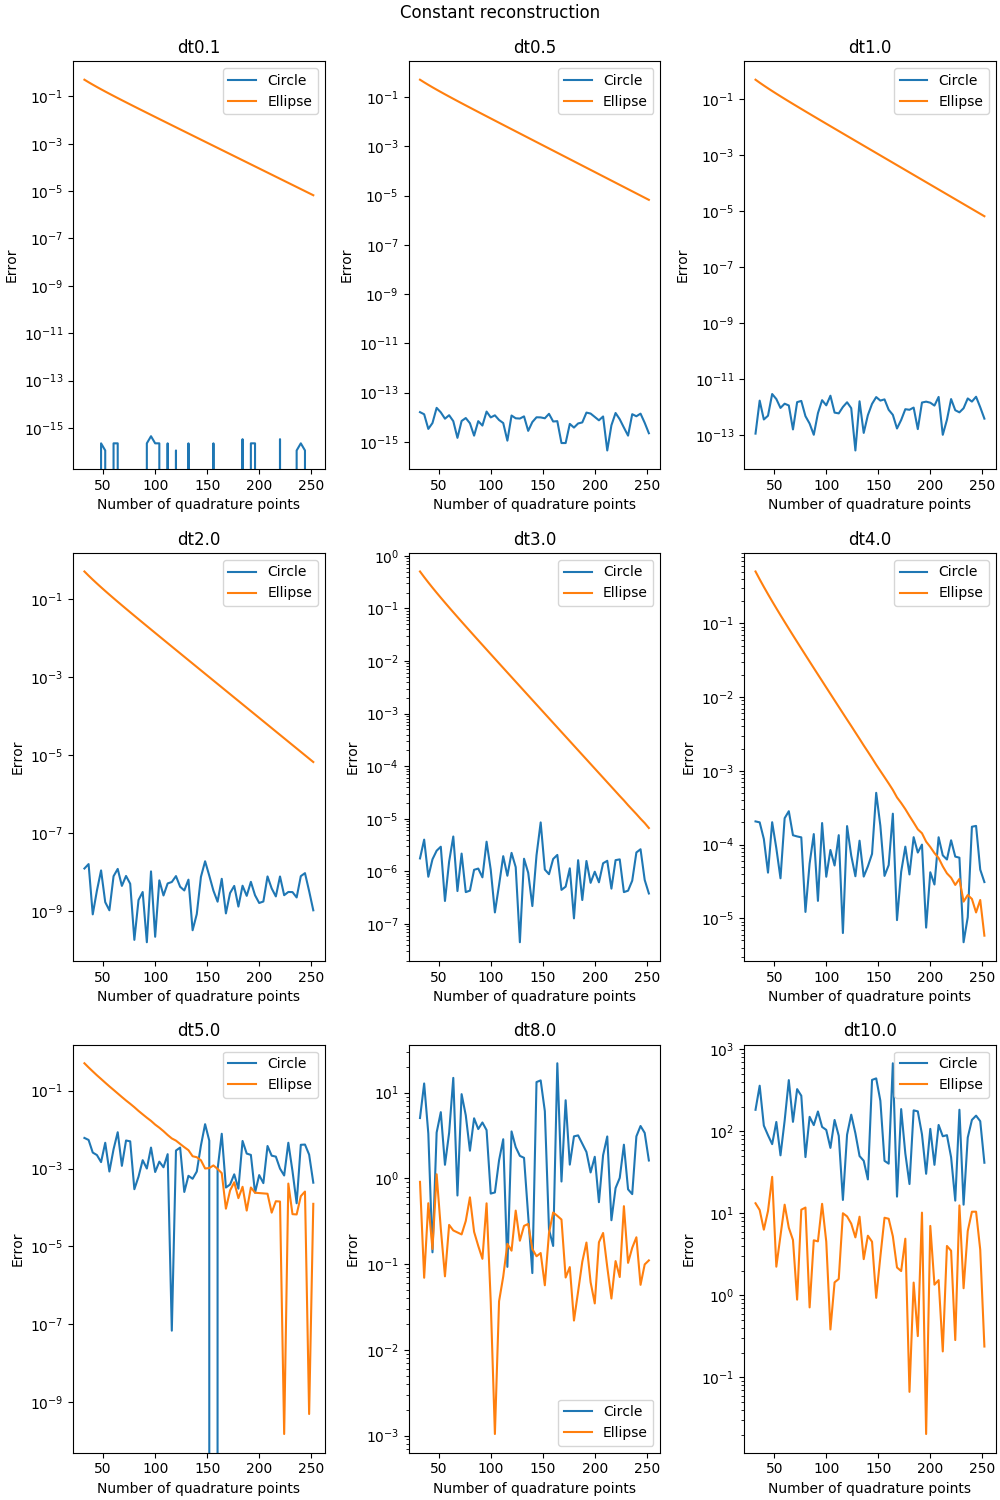
\includegraphics[scale=0.5]{const_recon_trunc16}
\label{fig:const_trunc16}
\caption{Absolute error in the numerical inversion of the function $\widehat{f}=1/s$ using truncated exponential with 16 terms, which should result in $f(t)=1$ for any $t$ ($dt$). }
\end{figure}

\clearpage
\section{Purely imaginary poles}

Let $f(t)=e^{i\alpha t}$, $\alpha \in \mathbb{R}$,  so that $\widehat{f}(s)=\frac{1}{s-i\alpha}$. We now apply the numerical inverse Laplace transform (NILT), on both circle and ellipse, with $\alpha$ values approaching the limit of the contour ($\gamma=10$). See results bellow. The same contours were used as before, with an ellipse with $\delta=0.5$ (see Fig \ref{fig:quad_elip_circ}).


\begin{figure}[h!]
\centering
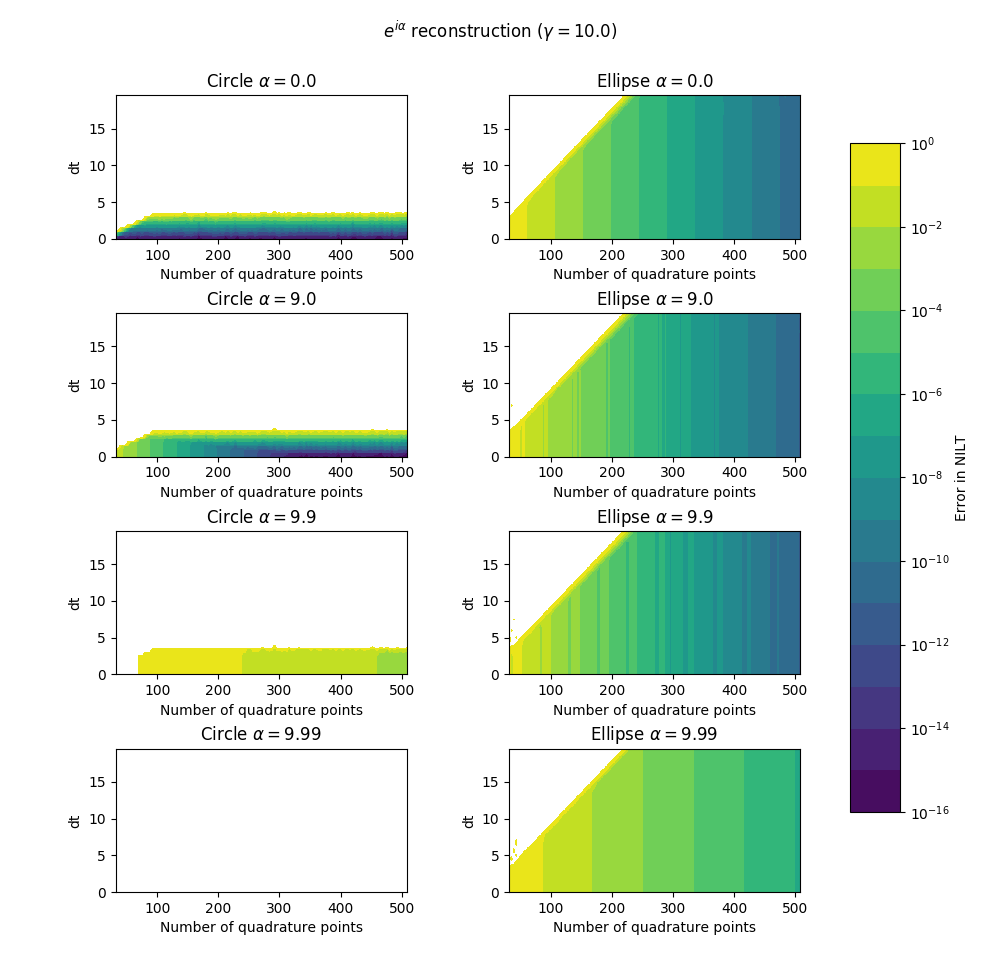
\includegraphics[scale=0.7]{nilt_expix_error}
\label{fig:const_trunc16}
\caption{Absolute error in the numerical inversion of the function $\widehat{f}(s)=1/(s-i\alpha)$, which should result in $f(t)=e^{i\alpha t}$ for varying $t$ ($dt$) and number of quadrature points. }
\end{figure}

\section{Relation to REXI }

The discussion above relies on the knowledge of the Laplace transform of the function one desires to invert. However, an analogous construction maybe done directly from the Cauchy Integration theorem:
\begin{equation}
f(x)=\frac{1}{2\pi i}\ointop_{C}\frac{f(z)}{z-x}dz,
\end{equation}
for $f$ holomorphic on $\mathbb{C}$, and the contour curve $C$ assumed to be closed and should be integrated in a counter-clockwise way, as before.

We can again chose $C$ to be the ellipse contour
\begin{equation}
s_n=\frac{\gamma i}{d}\left(re^{i\theta_n}+\frac{e^{-i\theta_n}}{r}\right), \quad n=1,2,..,N,
\end{equation}
and respectively the metric terms as
\begin{equation}
s'_n=-\frac{\gamma}{d}\left(re^{i\theta_n}-\frac{e^{-i\theta_n}}{r}\right),  \quad n=1,2,..,N,
\end{equation}
where $\theta_n=2\pi n/N$.

Therefore, the function $f$ can be approximated via,
\begin{equation}
f(x)=\frac{-1}{2\pi i} \int_{0}^{2\pi}\frac{f(s(\theta))}{s-x} s'(\theta) d\theta \approx 
\frac{-1}{2\pi i} \sum_{n=1}^{N}\frac{f(s_n)}{s_n-x} s'_ n \frac{2\pi}{ N},
\end{equation}
Simplifying,
\begin{equation}
f(x)\approx 
\frac{1}{ iN} \sum_{n=1}^{N}\frac{f(s_n)}{x-s_n} s'_ n =\frac{1}{N}\sum_{n=1}^{N}\frac{\beta_n}{x+\alpha_n},
\end{equation}
where
\begin{equation}
\beta_n=-if(s_n)s'_ n
\end{equation}
and 
\begin{equation}
\alpha_n=-s_n
\end{equation}
and also,
\begin{equation}
r=\sqrt{\frac{1-\delta/\gamma}{1+\delta/\gamma}},
\end{equation}
\begin{equation}
d=r^{-1}+r,
\end{equation}
and $\gamma$ is the largest attainable imaginary value and $\delta$ is the largest attainable real value of the ellipse, as discussed before.

\clearpage

\bibliographystyle{unsrtnat}
%\selectbiblanguage{english}

\bibliography{bibliography} 

\end{document}
